\section{Processi organizzativi}
    \subsection{Gestione processi}
		\subsubsection{Scopo}
		Lo scopo della gestione dei processi è di migliorare l'organizzazione e la cooperazione tra i membri del \glo{Gruppo}{gruppo}. La corretta implementazione del processo deve:
		\begin{itemize}
			\item stabilire le modalità di comunicazione del gruppo;
			\item definire i ruoli ed i compiti specifici;
			\item fornire la documentazione su strumenti di organizzazione e relative procedure.
		\end{itemize}

        \subsubsection{Comunicazioni}

            \paragraph{Interne}
                Per la comunicazione interna dei membri del gruppo, viene utilizzata l'applicazione \glo{Slack}{Slack} descritta in maniera piu dettagliata nella sezione \ref{sec:Slack}.

            \paragraph{Esterne}
				Per le comunicazioni esterne è stata creata la seguente mail:
				\begin{center}
					\mailzep{}
				\end{center}
				Il \responsabilediprogetto{} è la persona incaricata di inviare comunicazioni con questo indirizzo. Tutte le mail ricevute verranno inoltrate automaticamente ad ogni membro del gruppo a titolo informativo.
					% da valutare se inserire il canale {Slack} + il reindirizzamento alla persona specifica di riskapp
		%			
        \subsubsection{Incontri}
        %
            \paragraph{Interni}
            Il \responsabilediprogetto{} ha il compito di organizzare gli incontri interni rispettando la procedura descritta nella sezione \ref{sec:incontri_interni}{}.
	        Qualsiasi membro del gruppo può richiedere un incontro interno. Sarà compito del \responsabilediprogetto{} accettare o rifiutare la richiesta.
        	Al termine dell'incontro deve essere redatto un verbale, di cui si rimanda alla sezione \ref{sec:verbali} per la sua composizione in dettaglio.
            \paragraph{Esterni}
            Il \responsabilediprogetto{} ha il compito di organizzare gli incontri esterni con il proponente o committente seguendo la procedura descritta nella sezione \ref{sec:incontri_esterni}.
            Qualsiasi membro del gruppo può richiedere un incontro esterno. Sarà compito del \responsabilediprogetto{} accettare o rifiutare la richiesta.
            Al termine dell'incontro deve essere redatto un verbale, di cui si rimanda alla sezione \ref{sec:verbali} per la sua composizione in dettaglio.
        \subsubsection{Ruoli di progetto}
        	Ogni componente del gruppo deve ricoprire almeno una volta ciascuno dei ruoli previsti nello sviluppo del progetto. Nel \pdp{} vengono assegnati  compiti e ruoli che i membri del gruppo si impegnano a rispettare. Di seguito sono elencati i diversi incarichi, delineando per ciascuno mansioni e responsabilità.
			\paragraph{Responsabile di progetto}
			Il \responsabilediprogetto{} è la figura che rappresenta il gruppo e il progetto presso committente e proponente. Approva le scelte prese dal gruppo e se ne assume la responsabilità. La sua presenza segue tutta la durata del progetto.
			Le sue responsabilità sono:
			\begin{itemize}
				\item gestione delle risorse;
				\item approvazione della documentazione di progetto;
				\item analisi e mitigazione dei rischi;
				\item coordinamento e pianificazione delle attività di progetto seguendo il \pdp{}.
			\end{itemize}
			\paragraph{Amministratore di progetto}
			L'\amministratore{} è responsabile dell'ambiente di lavoro del gruppo, ne controlla l'efficienza e l'operatività.
			Le sue principali responsabilità sono:
			\begin{itemize}
				\item controllo delle versioni e configurazioni del prodotto;
				\item gestione del versionamento e dell'archiviazione della documentazione;
				\item risoluzione dei problemi inerenti la gestione di processi e risorse;
				\item controllo e miglioramento degli strumenti di lavoro e dell'infrastruttura;
				\item redazione e aggiornamento delle \ndp{}.
			\end{itemize}
			\paragraph{Analista}
			L'\analista{} ha il compito di esaminare e studiare attentamente il dominio del problema, la sua presenza non è necessaria per tutta la durata del progetto.
			Le sue responsabilità sono:
			\begin{itemize}
				\item capire il dominio di lavoro del cliente;
				\item analizzare e capire la natura del problema posto dal cliente;
				\item redigere lo studio di fattibilità e l'analisi dei requisiti.
			\end{itemize}
			\paragraph{Progettista}
			Il \progettista{} è responsabile di tutto ciò che riguarda la progettazione software. Deve avere conoscenze tecniche e tecnologiche aggiornate per la gestione del progetto.
			Le sue responsabilità sono:
			\begin{itemize}
				\item fornire una soluzione attuabile entro i limiti di tempo;
				\item descrivere il funzionamento del sistema a diversi livelli di dettaglio;
				\item effettuare scelte su aspetti tecnici del progetto, rendendolo efficiente, robusto e manutenibile.
			\end{itemize}
			\paragraph{Programmatore}
			Il \programmatore{} si occupa dell'attività di codifica. Le sue responsabilità sono:
			\begin{itemize}
				\item implementare le scelte dettate dal \progettista{}, senza apportare modifiche personali;
				\item documentare il codice prodotto;
				\item rispettare le convenzioni riportate nel presente documento;
				\item realizzare strumenti per verifica e validazione.
			\end{itemize}
			\paragraph{Verificatore}
			Il \verificatore{} è responsabile dell'attività di verifica. Deve avere una profonda conoscenza delle \ndp{} ed è presente per tutta la durata del progetto. Le sue responsabilità sono:
			\begin{itemize}
				\item controllare l'osservazione delle \ndp{} lungo tutte le attività del progetto stesso.
			\end{itemize}
		%
		\subsubsection{Strumenti}
		\paragraph{Slack}
		\label{sec:Slack}
		Slack è un servizio gratuito  di messaggistica professionale disponibile su piattaforme mobile, desktop e web. Le principali motivazioni che hanno portato il gruppo alla scelta di questo strumento sono:
		\begin{itemize}
			\item possibilità di integrazione con molti servizi, tra cui: \glo{Dropbox}{Dropbox}, \glo{GitHub}{GitHub}, \glo{Google Drive}{Google Drive}, bot etc. Vedi sezione \ref{sec:intSlack};
			\item possibilita di creare canali tematici personalizzati con la profilazione delle utenze e delle notifiche;
			\item utilizzato come ulteriore canale per comunicare con \riskapp{} in quanto anche loro lo utilizzano;
			\item possibilità di richiamare all'attenzione un membro del gruppo con il comando \hicode{@};
			\item possibilità di classificare  un commento  come "rilevante" tramite il comando \hicode{pin to};
			\item possibilità di inserire dei reminder sui messaggi;
			\item \glo{Cross-platform}{cross-platform} e \glo{Cross-device}{cross-device};
			\item interfaccia piu ricca e organizzata rispetto alle usuali applicazioni di messaggistica.
		\end{itemize}
		Lo spazio dedicato al gruppo si trova al seguente indirizzo:
		\begin{center}
			\url{https://zephyrus-swe.Slack.com/home}
		\end{center}
		\paragraph{Teamwork}\label{sec:teamwork}
		\glo{Teamwork}{Teamwork} è un'applicazione web di project management che permette di sfruttare le seguenti funzionalità principali:
		\begin{itemize}
			\item gestione dei task;
			\item gestione degli appuntamenti con scadenze a calendario;
			\item pianificazione del lavoro;
			\item rendiconto ore lavoro su intero progetto e/o su specifici task.
		\end{itemize}
		Le principali motivazioni che hanno portato il gruppo alla scelta di questo strumento sono:
		\begin{itemize}
			\item funzionalità essenziali gratuite ;
			\item alta portabilità ed accessibilità essendo fruibile via web;
			\item interfaccia semplice e funzionale.
		\end{itemize}
		Lo spazio di lavoro dedicato al gruppo di trova al seguente indirizzo:
		\begin{center}
			\url{https://swe2016.teamwork.com/}
		\end{center}
		\paragraph{Condivisione file}\label{sec:GoogleDrive}
		% 1)descrizione veloce dell'app
		\textit{Dropbox} è un servizio che offre la possibilità di salvare file su una piattaforma \glo{Cloud}{cloud} personale e mantenerli sincronizzati tra diversi dispositivi tramite un client.
		% 2)cosa ci permette di fare
		Il gruppo ha scelto Dropbox per gestire file che non necessitano versionamento,
		% 3) perche l'abbiamo scelta
		inoltre le principali motivazioni che ne hanno portato alla scelta sono:
		\begin{itemize}
			\item alta velocità nella sincronizzazione dei file;
			\item servizio già conosciuto e largamente utilizzato da tutti i membri del gruppo;
			\item lo spazio disponibile nella versione gratuita è sufficente per consentire una discreta quantità di file associati a questo progetto;
			\item alta portabilità e usabilità essendo cross-platform e cross-device.
		\end{itemize}
		% 4) indirizzo dove collegarsi
		Indirizzo per il download:
		\begin{center}
			\url{https://www.dropbox.com}
		\end{center}
		% 1)descrizione veloce dell'app
		\textit{Google Drive} è un servizio cloud, di memorizzazione e sincronizzazione online offerto da \textit{Google}. Il servizio comprende il \glo{File hosting}{file hosting}, il file sharing e la modifica collaborativa di documenti. Per accedere allo spazio condiviso è necessario che ogni membro sia prima aggiunto dal \responsabilediprogetto.
		% 2)cosa ci permette di fare
		Il gruppo ha scelto questo strumento per la possibilità di redigere documenti in maniera collaborativa come attività preliminare a fine organizzativo.
		% 3) perche l'abbiamo scelta
		Le principali motivazioni che hanno portato il gruppo alla scelta di questo strumento sono:
		\begin{itemize}
			\item servizio già conosciuto e utilizzato da tutti i membri del gruppo;
			\item gratuito;
			\item alta portabilità e usabilità essendo cross-platform e cross-device.
		\end{itemize}
		% 4) indirizzo dove collegarsi
		Lo spazio di lavoro dedicato al gruppo di trova al seguente link:
		\begin{center}
			\href{https://drive.google.com/drive/folders/0Bzwj6VVb_wEeYkhoYkdzVW5qQnM?usp=sharing}{Google Drive Zephyrus}
			% da valutare se inserire, xk si vede tutto, xò se un membro del gruppo deve accedere al gruppo su drive come farebbe? al limite mettere il link alla pagina drive "generica"
		\end{center}
		%
        \subsubsection{Procedure}
	        \paragraph{Organizzazione incontri interni}
	        \label{sec:incontri_interni}
	        L'organizzazione degli incontri interni deve essere svolta rispettando il seguente ordine:
	        \begin{enumerate}
	        	\item controllare il foglio condiviso su \glo{Google Drive}{Google Drive} \textit{Orari impegni ricorrenti};
	        	\item postare sul canale Slack \hicode{\#incontri-interni} alcune proposte di incontro, indicando: luogo, data e orario;
	        	\item assicurarsi che tutti i membri del gruppo abbiano espresso la preferenza; in caso contrario, entro 24 ore, contattarli telefonicamente;
	        	\item aggiungere l'evento nel calendario di \glo{Teamwork}{Teamwork} con le seguenti caratteristiche:
	        	\begin{itemize}
	        		\item \textbf{titolo evento:} Riunione interna;
	        		\item \textbf{dove:} data, ora inizio, ora fine;
	        		\item \textbf{dettagli:} luogo concordato, breve descrizione degli argomenti da trattare;
	        		\item \textbf{persone:} assegnare i partecipanti;
	        		\item \textbf{reminders:} assegnare dei promemoria se lo si ritiene necessario.
	        	\end{itemize}
	        \end{enumerate}
	        \paragraph{Organizzazione incontri esterni}
	        \label{sec:incontri_esterni}
	        L'organizzazione degli incontri esterni deve essere svolta rispettando il seguente ordine:
	         \begin{enumerate}
		        \item contattare il proponente per avere informazioni sulla sua disponibilità;
		        \item postare sul canale Slack \textit{\#incontri-esterni}{} alcune proposte di incontro, indicando: luogo, data e orario;
		        \item assicurarsi che tutti i membri del gruppo abbiano espresso la preferenza; in caso contrario, entro 24 ore, contattarli telefonicamente;
		        \item aggiungere l'evento nel calendario di Teamwork con le seguenti caratteristiche:
		        \begin{itemize}
		        	\item \textbf{Titolo evento:} Riunione esterna;
		        	\item \textbf{Dove:} data, ora inizio, ora fine;
		        	\item \textbf{Dettagli:} luogo concordato, breve descrizione degli argomenti da trattare;
		        	\item \textbf{Persone:} assegnare i partecipanti;
		        	\item \textbf{Reminders:} assegnare dei promemoria se lo si ritiene necessario.
		        \end{itemize}
	        \end{enumerate}
	        %
            \paragraph{Gestione dei ticket}\label{sec:procTicket}
            Accedere allo spazio Teamwork del gruppo, posizionandosi nella sezione \hicode{"All Task"} oppure tramite il seguente link: \url{https://swe2016.teamwork.com/#projects/140646/tasks}. Premere su \hicode{"Add Task"} per la creazione o sul nome di un task già esistente per la modifica.
            %
	            \subparagraph{Creazione di un ticket}\label{sec:creazioneticket}
	                La creazione di un ticket deve essere svolta dal \responsabilediprogetto{} rispettando il seguente ordine:
	                \begin{enumerate}
	                	\item inserimento titolo task;
	                	\item assegnazione delle persone incaricate al suo svolgimento;
	                	\item inserimento data prevista di completamento;
	                	\item inserimento del tempo stimato per il completamento;
	                	\item inserimento descrizione;
	                	\item inserimento priorità;
	                	\item selezionare eventuali dipendenze da altri task;
	                	\item inserimento di un \glo{Tag}{tag} che identifichi il ruolo delle persone incaricate;
	                	\item salvataggio task.
	                \end{enumerate}
	                Vedi figura \ref{fig:procassticket}.
	    	        \begin{figure}[h!]
	    		        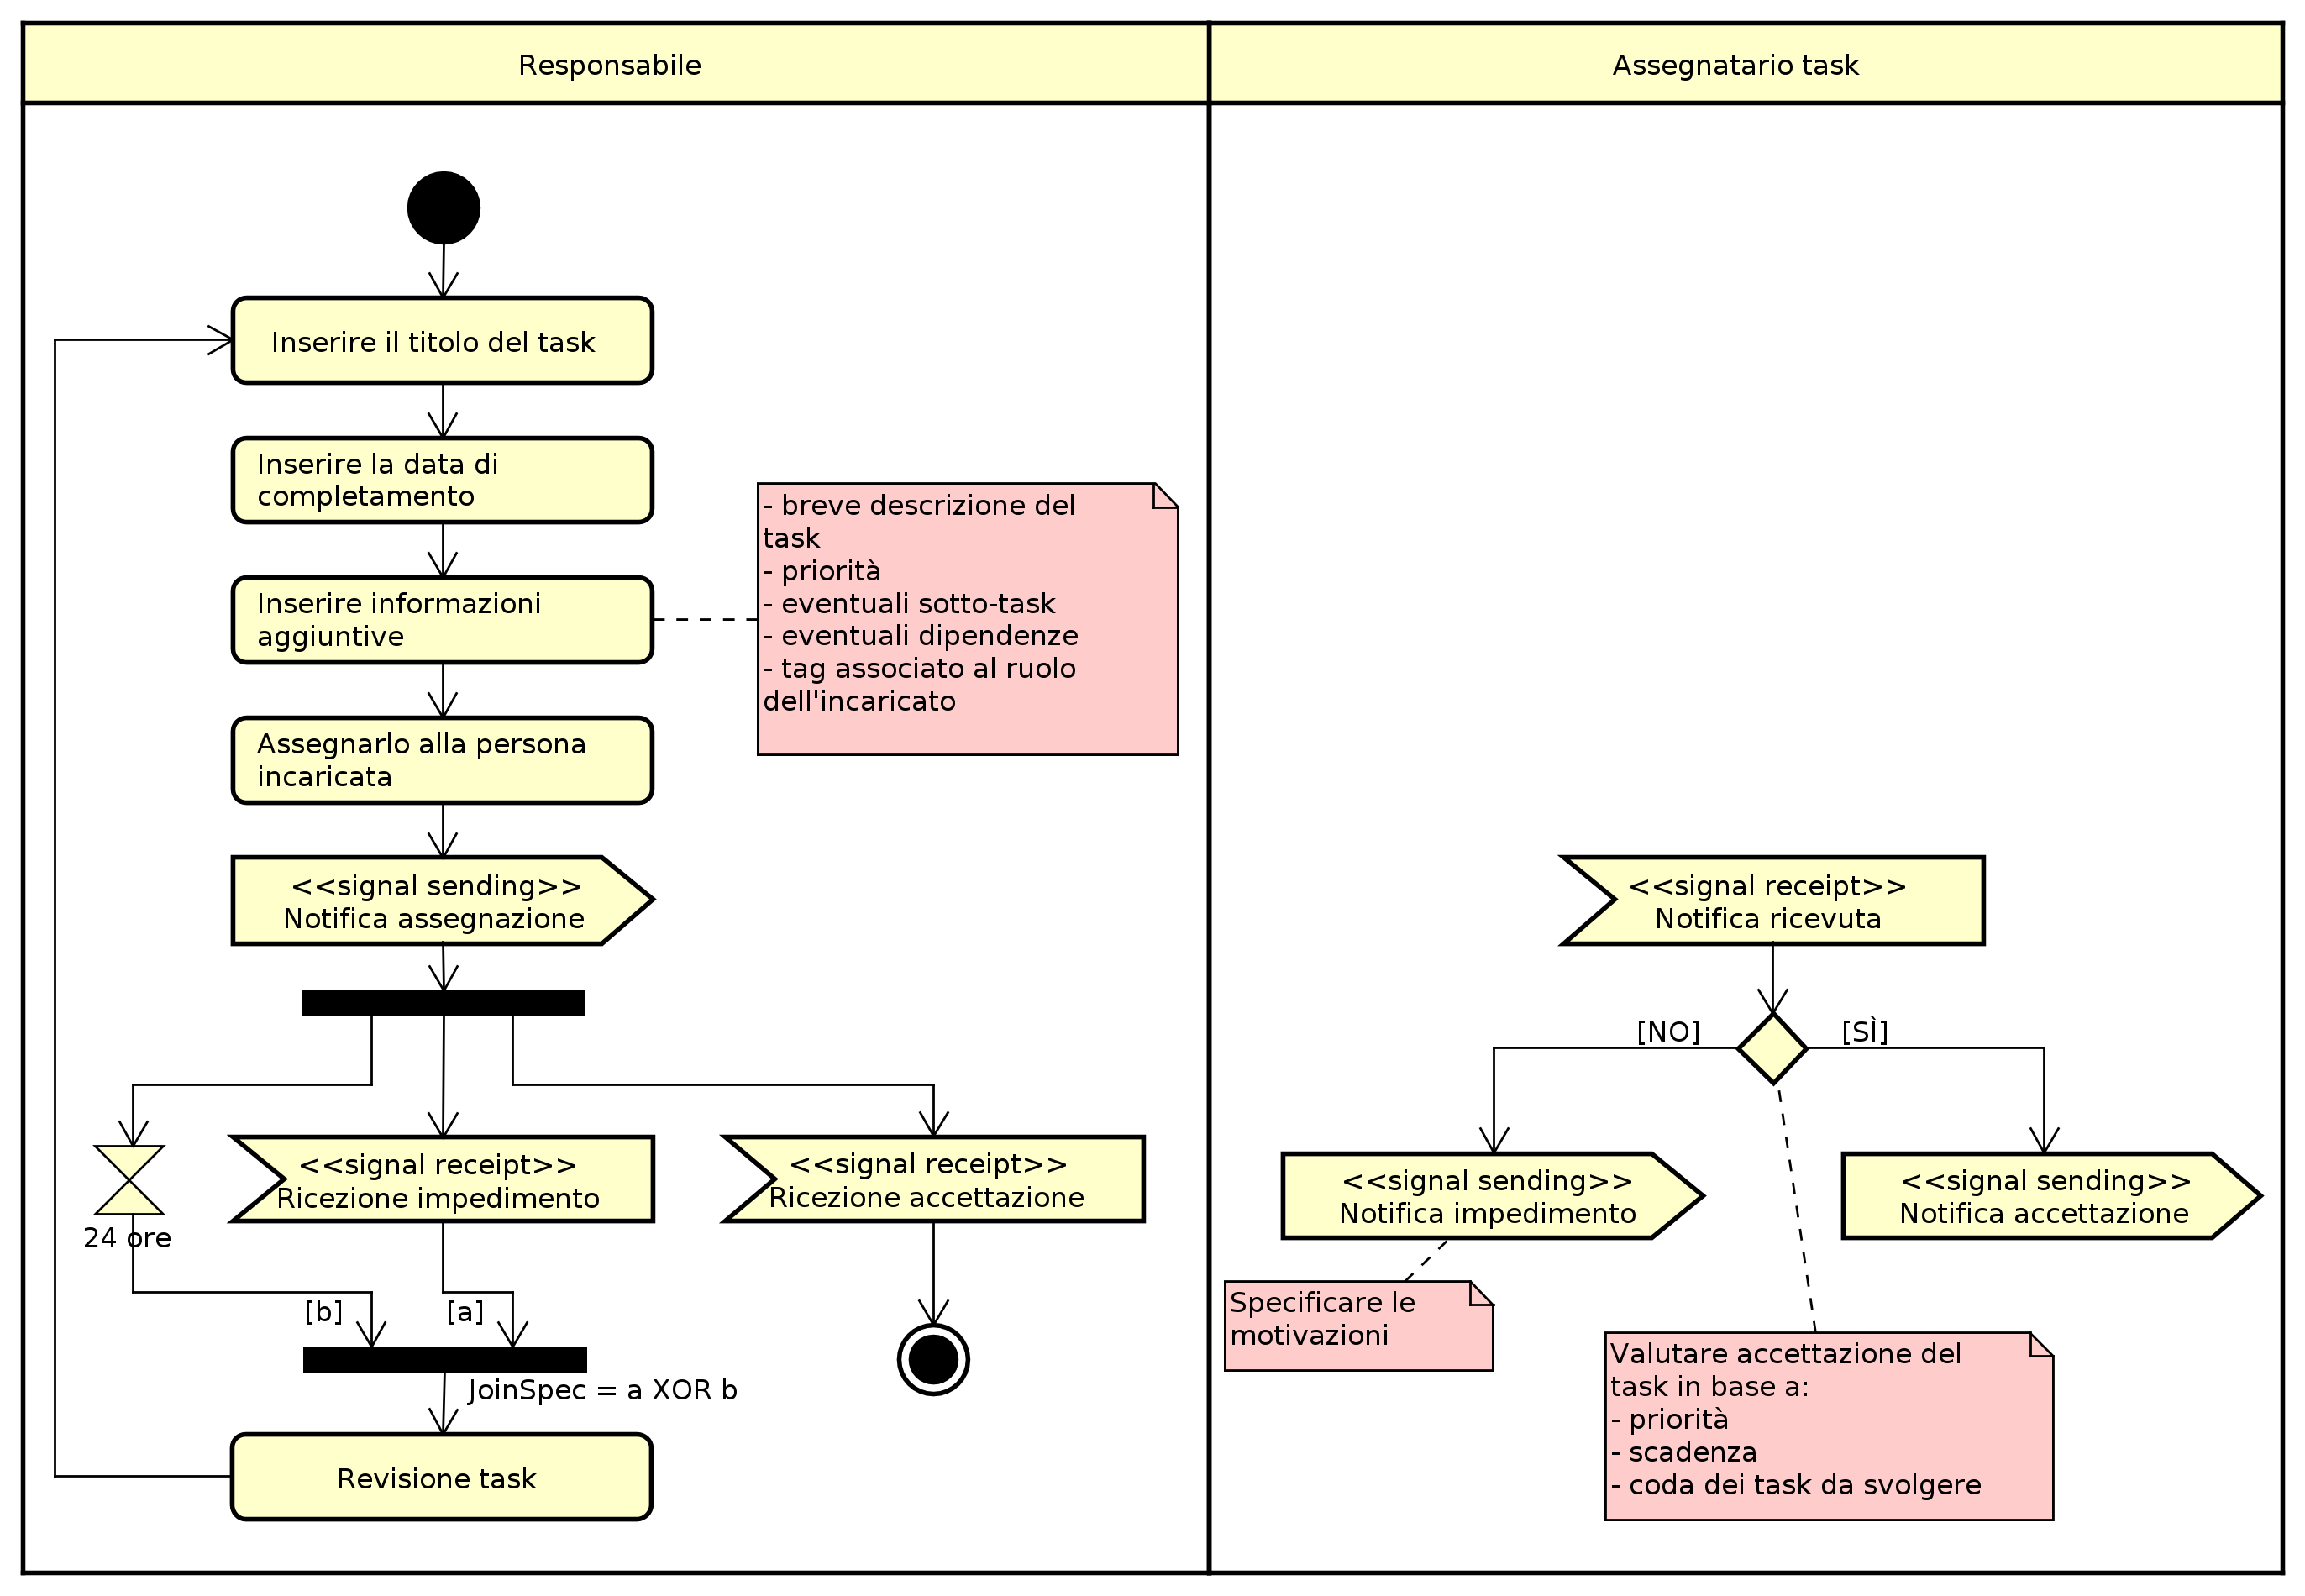
\includegraphics[width=\textwidth]{img/proc_ass_ticket.png}
	    		        \caption{Procedura assegnazione ticket. Riferita nella sezione \ref{sec:creazioneticket}}
	                    \label{fig:procassticket}
	    	        \end{figure}\mbox{}\\
	            \subparagraph{Modifica di un ticket}\label{sec:modificaticket}
	                La modifica di un ticket deve essere svolta rispettando il seguente ordine:
	                \begin{enumerate}
	                	\item ricerca del ticket da modificare;
	                	\item modifica di uno o più campi;
	                	\item verifica inserimento dei campi dati: titolo, assegnatario, descrizione e data di completamento;
	                	\item salvare le modifiche apportate.
	                \end{enumerate}
	                Vedi figura \ref{fig:procmodticket}.
	                    \begin{figure}[h!]
	                        \centering
	        	        	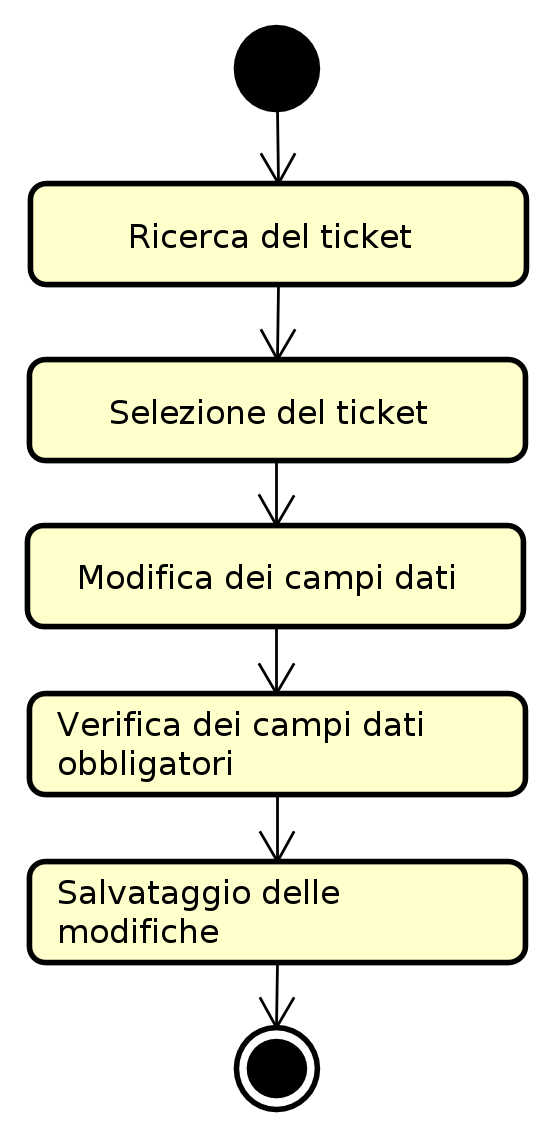
\includegraphics[width=0.3\textwidth]{img/proc_mod_ticket}
	                        \caption{Procedura modifica ticket. Riferita nella sezione \ref{sec:modificaticket}}
	                        \label{fig:procmodticket}
	        	        \end{figure}\mbox{}\\
	            \subparagraph{Chiusura di un ticket}\label{sec:chiusuraticket}
	            La chiusura di un ticket da parte dell'incaricato deve essere svolta rispettando la seguente procedura:
	            \begin{enumerate}
	            	\item ricerca del ticket da chiudere;
	            	\item aprire le proprietà del ticket e cliccare su \hicode{"Log time"};
	            	\item se il ticket è relativo ad un task di modifica di un documento:
	            	\begin{enumerate}
	            		\item eseguire un commit con solo l'aggiornamento del registro delle modifiche del documento;
	            		\item copiare il codice del commit ed inserirlo nella descrizione del task;
	            		\item eseguire il push delle modifiche.
	            	\end{enumerate}
	            	\item inserire il tempo speso per completare il task;
	            	\item selezionare \hicode{"Billable"} se il tempo speso è rendicontabile;
	            	\item selezionare \hicode{"Task is now complete"};
	            	\item cliccare su \hicode{"Log this time"}.
	            \end{enumerate}
	            Vedi figura \ref{fig:procChiusuraTicket}.\\\\
	            Una procedura automatica implementata nella chat Slack controllerà che il codice del commit inserito nel task sia presente nei messaggi inviati da GitHub, se così non fosse provvederà ad inviare un avviso al \responsabilediprogetto.
	        %
	        \begin{figure}[h!]
	        	\centering
	        	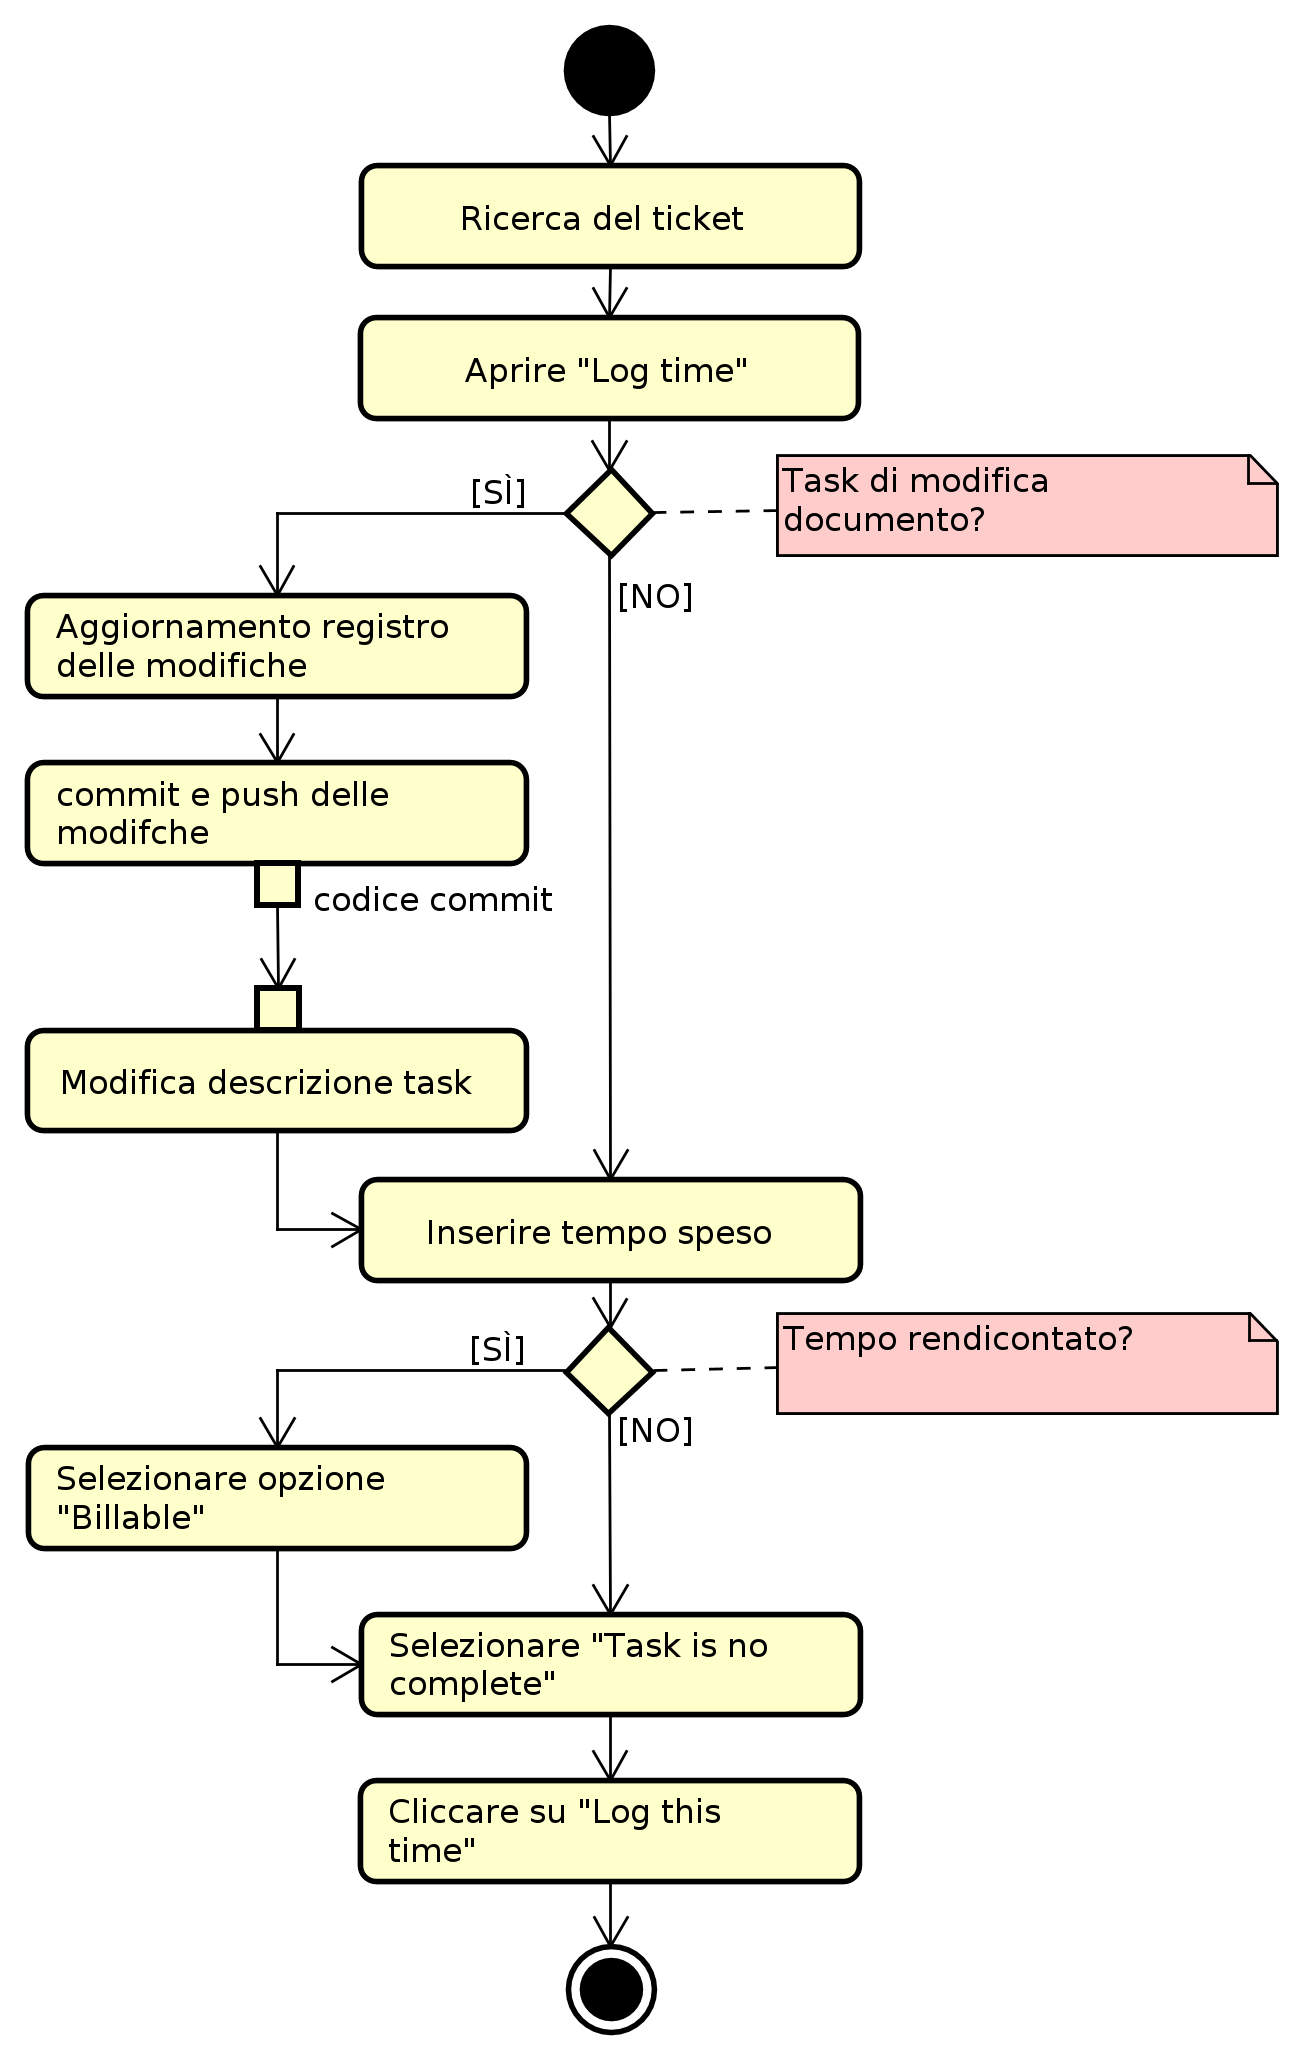
\includegraphics[width=0.6\textwidth]{img/proc_chiusura_ticket.png}
	        	\caption{Procedura chiusura ticket. Riferita nella sezione \ref{sec:chiusuraticket}}
	        	\label{fig:procChiusuraTicket}
	        \end{figure}\mbox{}\\
	        %
            \paragraph{Gestione delle milestone}
            Accedere allo spazio Teamwork del gruppo, posizionandosi nella sezione \textit{"Milestones"} oppure tramite il seguente link: \url{https://swe2016.teamwork.com/#/projects/140646/milestones/upcoming}. Premere su \textit{"Add \glo{Milestone}{Milestone}"} per la creazione o sul nome di una milestone esistente per la modifica.
            \subparagraph{Creazione milestone}\label{sec:creazionemilestone}
                La creazione di una milestone deve essere svolta rispettando il seguente ordine:
    			\begin{enumerate}
    				\item inserimento titolo milestone;
    				\item inserimento data;
    				\item assegnazione persone coinvolte;
    				\item assegnazione reminders;
    				\item inserimento descrizione;
    				\item salvataggio milestone.
    			\end{enumerate}
                Vedi figura \ref{fig:procinsmilestone}.
    			\begin{figure}[h!]
                    \centering
    				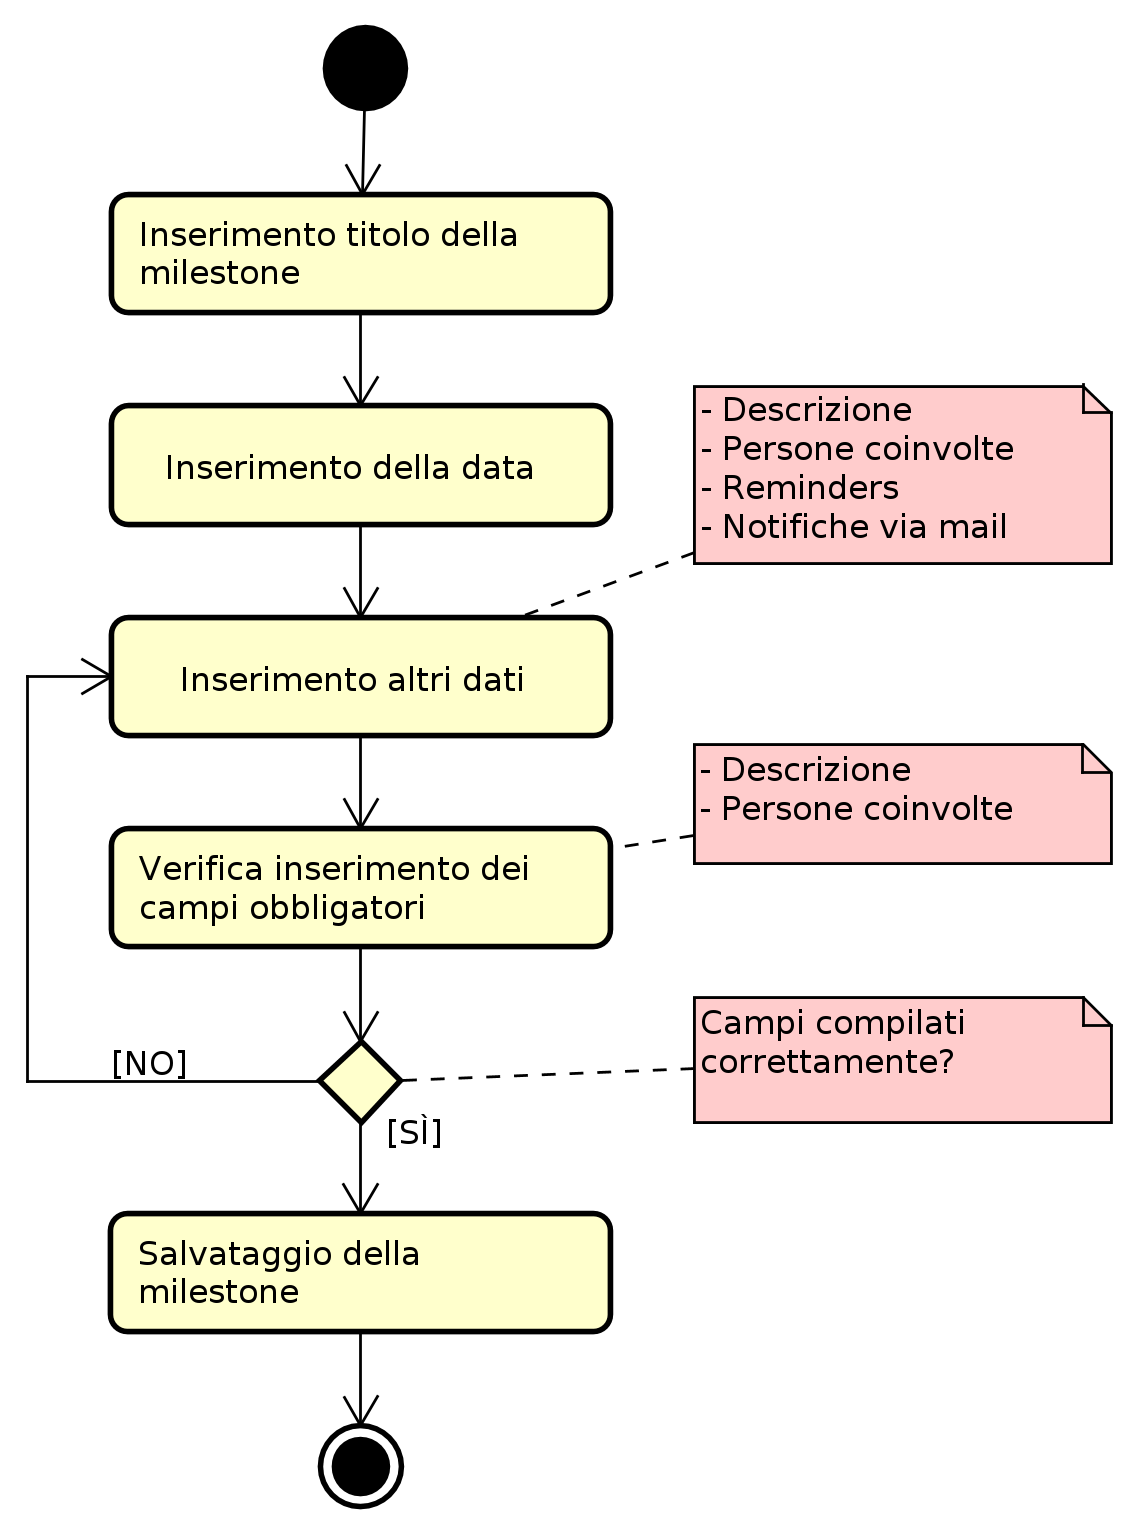
\includegraphics[width=0.5\textwidth]{img/proc_ins_milestone}
    				\caption{Procedura inserimento milestone. Riferita nella sezione \ref{sec:creazionemilestone}}
                    \label{fig:procinsmilestone}
    			\end{figure}\mbox{}\\
            \subparagraph{Modifica milestone}\label{sec:modificamilestone}
			La modifica di una milestone deve essere svolta rispettando il seguente ordine:
    			\begin{itemize}
    				\item selezione milestone;
    				\item modifica di uno o più campi dati;
    				\item verifica inserimento dei campi dati: titolo, data, descrizione e assegnatari;
    				\item salvataggio milestone.
    			\end{itemize}
                Vedi figura \ref{fig:procmodmilestone}.
        		\begin{figure}[h!]
                    \centering
        			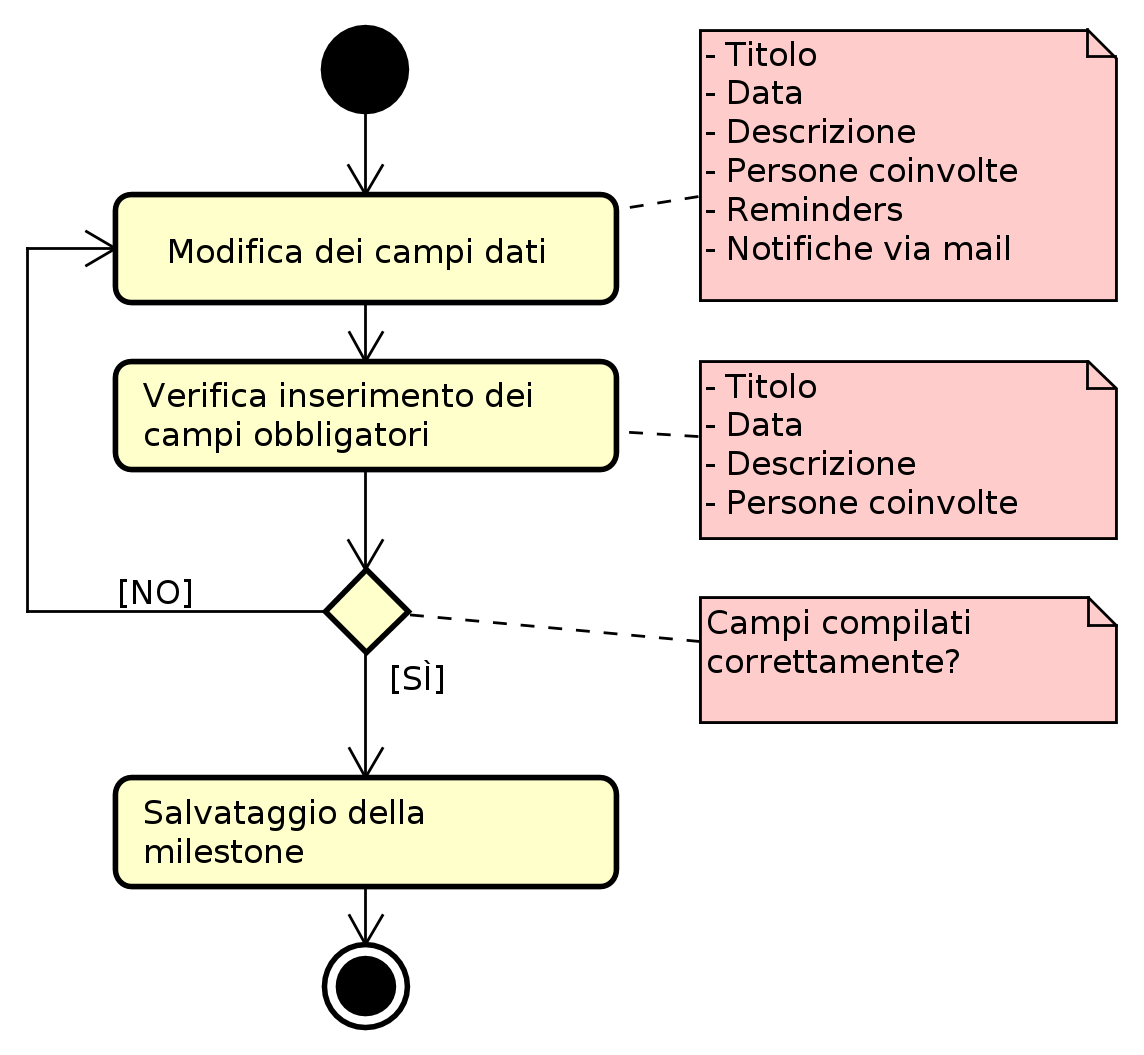
\includegraphics[width=0.5\textwidth]{img/proc_mod_milestone}
        			\caption{Procedura modifica milestone. Riferita nella sezione \ref{sec:modificamilestone}}
                    \label{fig:procmodmilestone}
        		\end{figure}\mbox{}\\
        %
       	\paragraph{Creazione nuovo canale Slack}\label{sec:CreaCanale}
		La creazione di un nuovo canale Slack può essere fatta solo da parte del \responsabile{} e deve rispettare il seguente ordine:
		\begin{enumerate}
			\item effettuare il login su Slack nel sito o nell'applicazione, con l'utente \textit{zephyrus.swe};
			\item cliccare nel menù di sinistra la voce \hicode{CHANNELS};
			\item cliccare il pulsante \hicode{New Channel};
			\item scegliere se rendere il canale pubblico o privato;
			\item scegliere il nome del canale;
			\item compilare l'eventuale descrizione riguardo la tematica del canale;
			\item inserire i nomi delle persone che si desidera invitare;
			\item cliccare sul bottone \hicode{Create Channel}.
		\end{enumerate}
		Vedi figura \ref{fig:ProCreaCanale}.
		\begin{figure}[h!]
			\centering
			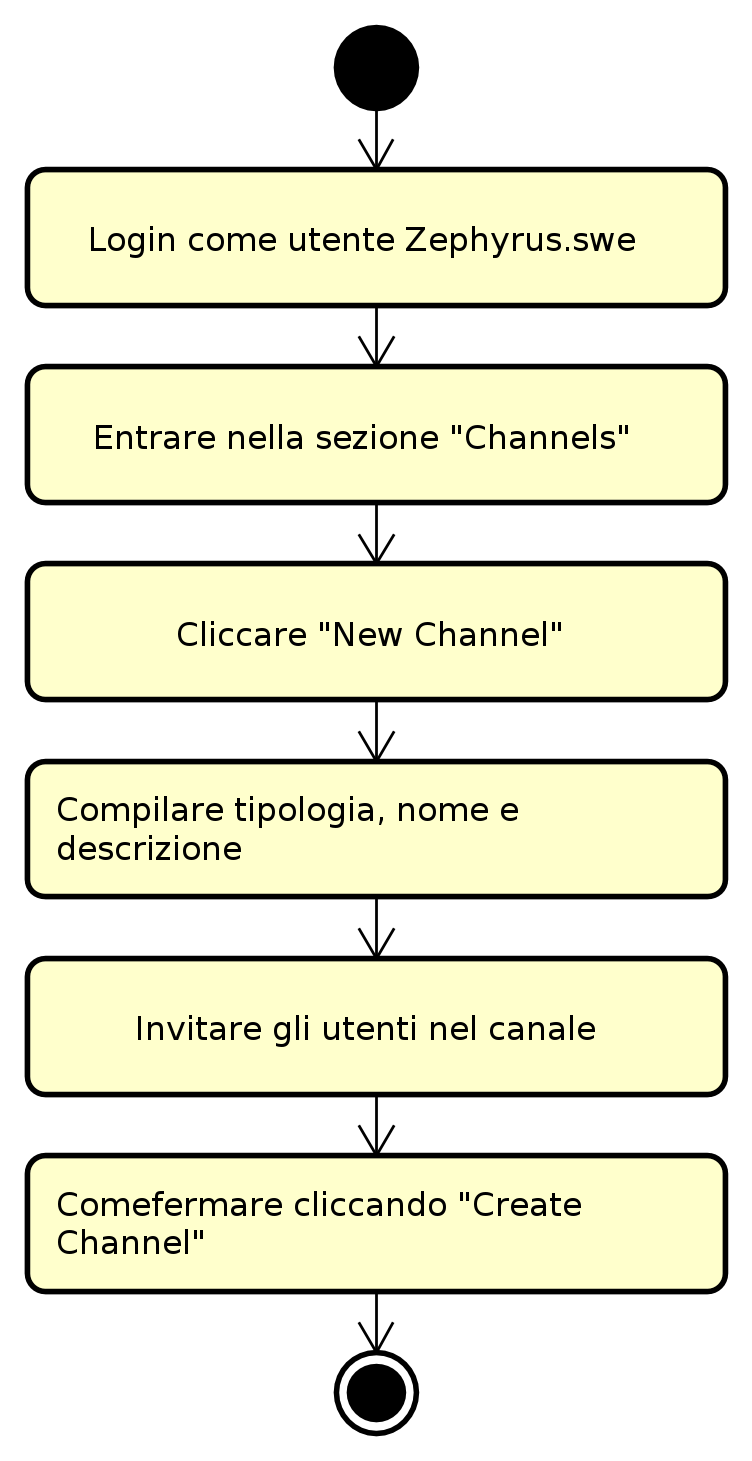
\includegraphics[width=0.3\textwidth]{img/CreazioneCanaleSlack}
			\caption{Procedura di creazione di un canale Slack. Riferita nella sezione \ref{sec:CreaCanale}}
			\label{fig:ProCreaCanale}
		\end{figure}\mbox{}\\
		%
		\paragraph{Modifica impostazioni canale Slack}\label{sec:ModCanale}
		In un canale Slack si possono modificare varie impostazioni, tra cui: 
		\begin{itemize}
			\item invitare o rimuovere membri;
			\item preferenze di notifica;
			\item integrare app esterne;
			\item silenziare il canale;
			\item uscire dal canale.
		\end{itemize}
		Tranne la prima, tutte le altre sono a discrezione dell'utente. Di seguito si presenta la procedura eseguibile solo dal \responsabile{} per aggiungere un membro al canale. 
		\begin{enumerate}
			\item effettuare il login su Slack nel sito o nell'applicazione, con l'utente \hicode{zephyrus.swe};
			\item cliccare nel canale che si desidera apportare modifiche;
			\item cliccare il pulsante con l'icona a forma di ingranaggio e successivamente \hicode{Invite team Members};
			\item inserire il nickname della persona che si vuole aggiungere;
			\item cliccare sul bottone \hicode{Invite}.
		\end{enumerate}
		N.B. Per poter visualizzare il nome della persona da aggiungere è necessario che quest'ultima faccia già parte del Team su Slack, in caso contrario bisogna invitarla tramite indirizzo mail.
		Vedi figura \ref{fig:ProModChannel}.
		\begin{figure}[h!]
			\centering
			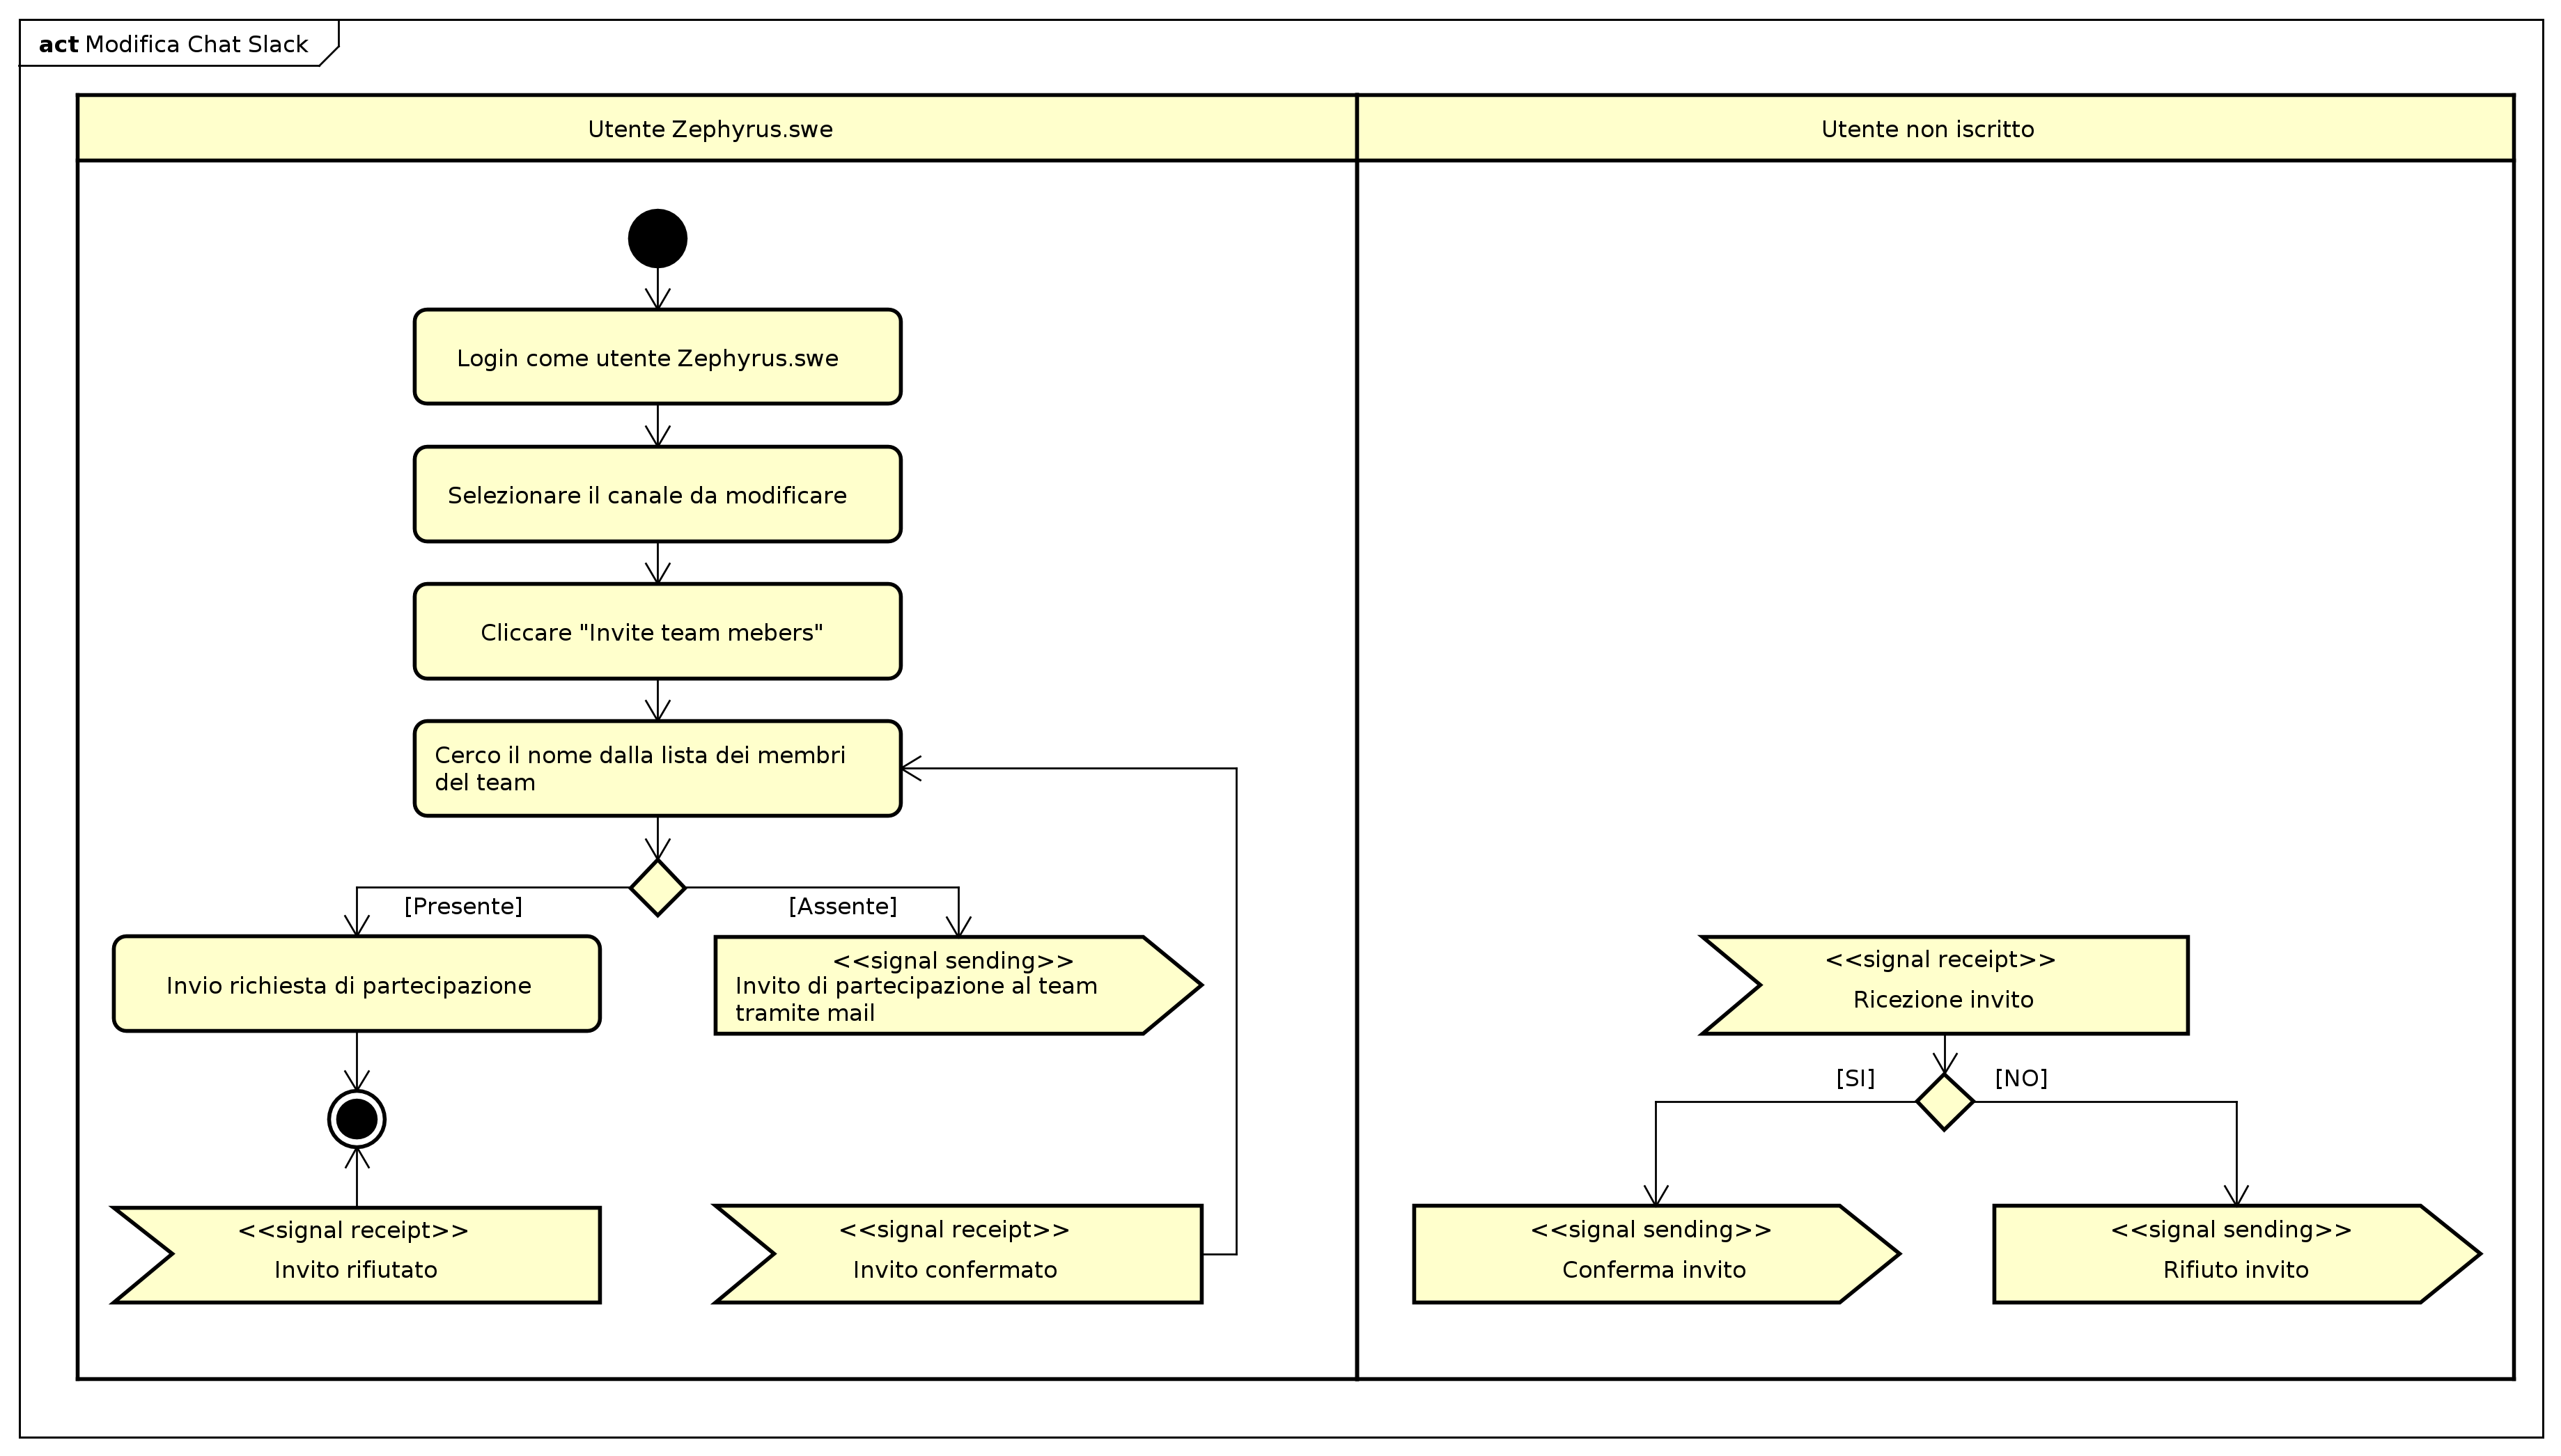
\includegraphics[width=\textwidth]{img/ProModChannel}
			\caption{Procedura di creazione di un canale Slack. Riferita nella sezione \ref{sec:ModCanale}}
			\label{fig:ProModChannel}
		\end{figure}\mbox{}\\	
	
        
    \subsection{Gestione delle infrastrutture}
        \subsubsection{Scopo}
        Lo scopo del processo di gestione delle infrastrutture è di stabilire e mantenere le infrastrutture e gli strumenti necessari allo svolgimento dei processi durante lo svolgimento del progetto. La corretta implementazione del processo deve:
        \begin{itemize}
            \item fornire un ambiente di lavoro idoneo;
            \item garantire il funzionamento di tutte le infrastrutture necessarie;
            \item indicare il corretto utilizzo delle infrastrutture.
        \end{itemize}

		\subsubsection{Ambiente di sviluppo}
		L'\amministratore{} ha il compito di decidere l'ambiente ottimale per lo sviluppo e il test dell'applicazione. Se necessario è possibile coinvolgere il proponente nella decisione, in questo caso sarà compito del \responsabilediprogetto{} organizzare le riunioni o i contatti necessari.
		Una volta deciso l'ambiente di sviluppo l'\amministratore{} dovrà indicare a tutti i membri del gruppo le procedure necessarie per il suo corretto utilizzo, eventuali modifiche o aggiornamenti dovranno essere segnalati tempestivamente tramite gli appositi canali di comunicazione.

        \subsubsection{Aggiornamento applicazioni}
        L'\amministratore{} ha il compito di informare tutti i membri del gruppo di eventuali aggiornamenti disponibili per applicazioni in uso e se una loro installazione potrebbe generare incompatibilità con altri strumenti.
        Inoltre deve mantenere aggiornato, situato nello spazio Google Drive, il documento condiviso:
        \begin{center}
        	\texttt{Strumenti utilizzati}
        \end{center}
        contenente le versioni degli strumenti installati per ogni membro del gruppo.
        
        \subsubsection{Gestione account e password}
        L'\amministratore{} ha il compito di mantenere aggiornato il documento contenente le informazioni riguardanti gli account degli strumenti e dei siti in uso per lo svolgimento del progetto, comunicando eventualmente le variazioni ai membri del gruppo interessati. Inoltre deve monitorare l'utilizzo degli spazi per la condivisione dei file per assicurarsi che vengano utilizzati unicamente per gli scopi del progetto e per garantire che tutti i membri del gruppo possano accedervi senza limitazioni.
        
		\subsubsection{Gestione comunicazioni}
		L'\amministratore{} ha il compito di controllare e gestire i canali presenti nella chat Slack per mantenere un livello di conversazione accettabile e costruttivo fra tutti i membri del gruppo e per garantire che la chat non venga utilizzata impropriamente.
		Nello specifico l'\amministratore{} dovrà:
		\begin{itemize}
			\item assicurarsi che il linguaggio utilizzato sia rispettoso di tutti i membri del gruppo e consono all'ambiete di lavoro;
			\item assicurarsi che ogni canale venga utilizzato unicamente allo scopo preposto;
			\item se necessario, creare nuovi canali e invitarvi i membri del gruppo che li dovranno utilizzare;
			\item archiviare canali non più utilizzati se ritenuto opportuno;
			\item eliminare messaggi ritenuti inopportuni o non in linea con le indicazioni di cui sopra;
			\item gestire eventuali estensioni di Slack;
			\item farsi carico di eventuali lamentele o segnalazioni da parte dei membri del gruppo e riportarle al \responsabilediprogetto{} se necessario.
		\end{itemize}
	%
	\subsubsection{Strumenti}
	\paragraph{Integrazioni Slack} \label{sec:intSlack}
	L'\amministratore{} ha il compito di controllare e gestire le integrazioni della chat Slack:
	\begin{itemize}
		\item \textbf{Teamwork:} il canale \hicode{\#task} dovrà contenere tutti i messaggi provenienti da Teamwork e relativi alla creazione, modifica e chiusura dei ticket;
		\item \textbf{GitHub:} il canale \hicode{\#dev} dovrà contenere tutti i messaggi provenienti dai commit eseguiti sui repository git utilizzati;
		\item \textbf{Condivisione:} il canale \hicode{\#share} dovrà contenere tutti i messaggi provenienti dalle modifiche eseguite su Dropbox o GoogleDrive.
	\end{itemize}
	%
	\paragraph{Node.js} \label{nodejs}
	\glo{Node.js}{Node.js} è una piattaforma event-driven per il motore \glo{JavaScript}{JavaScript} V8, disponibile sulle principali piattaforme, anche se maggiormente performante su sistemi operativi UNIX-like.
	L'indirizzo per il download e la documentazione:
	\begin{center}
		\url{https://nodejs.org/en/download/}
	\end{center}
	%
	\paragraph{npm}
	npm (node package manager) è il gestore di pacchetti di default utilizzato da Node.js. Questo strumento consente  l'installazione e la gestione di moduli esterni che forniscono funzionalità aggiuntive al sistema node di base, risolvendo varie dipendenze.
	Le principali motivazioni che hanno portato il gruppo alla scelta di questo strumento sono:
	\begin{itemize}
		\item larga diffusione;
		\item più di 400.000 pacchetti installabili;
		\item ampia documentazione.
	\end{itemize}
	Indirizzo per il download e la documentazione:
	\begin{center}
		\url{https://www.npmjs.com}
	\end{center}
	\paragraph{Sistemi operativi}
	I membri del gruppo operano sui seguenti sistemi operativi:
	\begin{itemize}
		\item \glo{Linux}{Linux} distribuzioni: Debian v8.0, Ubuntu v16.04 e superiori;
		\item \glo{Windows}{Windows} versione: 10;
		\item \glo{MacOS}{MacOS} versione: 10.12.
	\end{itemize}
	%
	\paragraph{VirtualBox}
	% 1)descrizione veloce dell'app
	VirtualBox è un'applicazione opensource e gratuita sviluppata da Oracle per l'esecuzione di macchine virtuali,
	% 2)cosa ci permette di fare
	permette quindi di eseguire ed utilizzare all'interno di qualsiasi computer un sistema virtualizzato con caratteristiche diverse dal sistema che lo ospita.
	% 3) perche l'abbiamo scelta
	L'applicazione è stata scelta di comune accordo con il proponente, che fornirà l'immagine di una macchina virtuale con le caratteristiche necessarie per poter essere utilizzata come ambiente di sviluppo e test.\\
	% 4) indirizzo dove collegarsi
	VirtualBox è disponible per tutti i principali sistemi operativi e la sua installazione non prevede procedure particolari. La versione utilizzata è quella stabile, oltre all'applicazione è necessario installare anche l'\textit{Extension Pack}. Tutte le informazioni necessarie al download e all'installazione possono essere trovate al seguente indirizzo:\\
	\begin{center}
		\url{https://www.virtualbox.org/wiki/Downloads}
	\end{center}
	%
	\paragraph{FileZilla Client}
	% 1)descrizione veloce dell'app
	FileZilla Client è un software opensource cross-platfom che permette il trasferimento di file in rete attraverso il protocollo FTP.
	
	Il programma è disponibile per i sistemi operativi Linux, Microsoft Windows, e macOS. Tra i vari protocolli supportati, oltre all'FTP c'è l'SFTP, e l'FTP su SSL/TLS.
	% 3) perche l'abbiamo scelta
	Le principali motivazioni che hanno portato il gruppo alla scelta di questo strumento sono:
	\begin{itemize}
		\item applicazione semplice e leggera;
		\item già conosciuta da molti membri del gruppo.
	\end{itemize}
	Indirizzo per il download e la documentazione:
	\begin{center}
		\url{https://filezilla-project.org/download.php?type=client}
	\end{center}
	%	
	\subsubsection{Procedure}
	\paragraph{Backup}
	Con cadenza mensile l'\amministratore{} deve eseguire un backup su dispositivo esterno dei seguenti dati:
	\begin{itemize}
		\item \glo{Database}{database} \glo{Trender}{Trender};
		\item repository Documenti;
		\item repository Codice;
		\item cartella Dropbox.
	\end{itemize}
	%
	\paragraph{Configurazione VirtualBox}
	La macchina virtuale fornita da \riskapp{} deve essere configurata per poter consentire un agevole ambiente di sviluppo e test per il progetto.
	
	Inizialmente si configura la VirtualBox precedentemente installata seguendo i seguenti passi:
	\begin{enumerate}
		\item aprire VirtualBox;
		\item entrare nel menù \hicode{File -> Preferences -> Network -> NAT Networks};
		\item cliccare sul bottone \hicode{"+" (Add)};
		\item cliccare sul bottone \hicode{Edit};
		\item cliccare su \hicode{"Port Forwarding"};
		\item selezionare \hicode{IPv4};
		\item cliccare sul bottone \hicode{"+" (Add)};
		\item editare i campi in modo da avere le seguenti due regole:  \\
		\begin{table}[H]
			\centering
			\begin{tabular}{|llllll|}
				\hline
				Name & Protocol & Host IP & Host Port & Guest IP & Guest Port \\ \hline
				Rule 1 & TCP & 127.0.0.1 & 10080 & 10.0.2.15 & 80 \\ \hline
				Rule 2 & TCP & 127.0.0.1 & 10022 & 10.0.2.15 & 22 \\ \hline
			\end{tabular}
		\end{table}
		\item chiudere le finestra cliccando su \hicode{Ok}.
	\end{enumerate}
	In questo modo si può testare il sito dal browser del proprio PC invece che da quello della macchina virtuale, aprendo il browser e digitando l'URL \url{http://localhost:10080}.
	%
	Successivamente si procede con la configurazione della macchina virtuale precedentemente installata come descritto nella sezione \ref{installazioneMacchinaVirtuale} rispettando i seguenti passi:
	\begin{enumerate}
		\item aprire Virtualbox;
		\item cliccare con il tasto destro sulla macchina virtuale "Zephyrus" \hicode{Settings -> Network};
		\item impostare il campo "Connect to:" a \hicode{Nat Network};
		\item impostare il campo "Name" a \hicode{NatNetwork};
		\item chiudere le finestre cliccando sul bottone \hicode{Ok};
		\item avviare la macchina virtuale premendo sul bottone \hicode{Start}.
	\end{enumerate}
	%
	\paragraph{Installazione macchina virtuale} \label{installazioneMacchinaVirtuale}
	\begin{enumerate}
		\item Scaricare il file con l'immagine dal seguente link:
		\begin{center}
			\url{https://www.satellite1.info/u/Zephyrus.ova}
		\end{center}
		\item aprire l'applicazione VirtualBox sul proprio computer;
		\item aprire il menù \hicode{File} e selezionare \hicode{Import Appliance};
		\item selezionare il file \hicode{Zephyrus.ova} scaricato nel punto 1 e cliccare su \hicode{Next};
		\item cliccare su \hicode{Import} e attendere la fine del processo;
		\item terminata l'importazione fare click destro sulla nuova macchina virtuale presente nell'elenco a sinistra e selezionare \hicode{Settings};
		\item selezionare la sezione \hicode{Network};
		\item nella tab \hicode{Adapter 1} modificare l'opzione \hicode{Attached to: NAT} e cliccare \hicode{OK};
		\item la macchina virtuale è ora pronta all'uso.
	\end{enumerate}
	%
	\paragraph{Configurazione FileZilla Client per invio file su macchina virtuale}
	Configurazione per l'invio dei file alla macchina virtuale Zephyrus tramite SFTP.
	\begin{enumerate}
		\item aprire FileZilla;
		\item entrare nel menù \hicode{File -> gestore siti};
		\item cliccare sul bottone \hicode{Nuovo sito};
		\item editare i seguenti campi:
			\begin{itemize}
				\item \hicode{Host: sftp://127.0.0.1} 
				\item \hicode{Username: admin}
				\item \hicode{Password: admin}
				\item \hicode{Port: 10022}
				\item \hicode{Protocollo: SFTP - SSH File Transfer Protocol}
				\item \hicode{Tipo di accesso: normale}
			\end{itemize}
		\item premere il bottone \hicode{Ok} per salvare le modifiche.
	\end{enumerate}
	Il file js caricato ora da riskapp è:
	\begin{center}
		\url{/home/admin/ayako/frontend/static/akane/akane.js}
	\end{center}
	che è un link verso:
	\begin{center}
		\url{/opt/ayako/ayako/ayako/frontend/static/akane/akane.js}
	\end{center}
	ora basta solamente sovrascrivere il loro file con quello prodotto dal gruppo \zephyrus.
	%
	\paragraph{Segnalazioni e richieste} \label{sec:procRichieste}
	Qualora un componente del gruppo voglia inviare una segnalazione o una richiesta riguardo l'infrastruttura o gli strumenti utilizzati essa dovrà essere fatta tramite il sistema di ticketing nel seguente modo:
	\begin{enumerate}
		\item creare un nuovo task su teamwork;
		\item inserire uno dei seguenti tag nel titolo del task:
		\begin{itemize}
			\item \cit{[NCR]} per richiedere l'inserimento di un nuovo comando personalizzato nel template \LaTeX;
			\item \cit{[RICHIESTA]} per una richiesta generica;
			\item \cit{[SEGNALAZIONE]} per segnalare un problema o un'anomalia;
		\end{itemize}
		\item inserire il ruolo del richiedente della modifica nel corpo del task;
		\item spiegare in maniera concisa la natura della richiesta e le sue motivazioni nel corpo del task;
		\item assegnare il task all'\amministratore;
		\item solamente se necessario impostare una data di scadenza del task.
	\end{enumerate}
	Una volta ricevuto il task l'\amministratore{} potrà:
	\begin{itemize}
		\item accettare o rifiutare direttamente la richiesta motivando la scelta;
		\item coinvolgere se necessario il \responsabilediprogetto{} assegnandogli il task in questione con eventuali commenti.
	\end{itemize}
	Richieste inviate in maniera diversa da quanto descritto in questa procedura non verrano prese in considerazione.
	%
	\subsection{Apprendimento}
	\subsubsection{Scopo}
	Lo scopo del processo di apprendimento è di garantire che ogni membro del gruppo abbia conoscenze e capacità sufficienti per svolgere le attività assegnatagli. Nel caso in cui un componente del gruppo ritenga di non essere in grado di svolgere un task dovrà segnalarlo immediatamente al \responsabilediprogetto{} che dovrà organizzare le attività necessarie all'apprendimento.
	%
	\paragraph{Guide e documentazione} \label{sec:guidalatex}
	Riguardo la formazione, tutti i membri del gruppo devono procedere in modo autonomo con lo studio delle tecnologie che verranno utilizzate nel corso del progetto, prendendo come riferimento, oltre al materiale indicato nella sezione \ref{sec:riferimenti}, anche la seguente documentazione:
	\begin{itemize}
		\item \textbf{Documentazione ufficiale React:} \url{https://facebook.github.io/react/docs/hello-world.html};
		\item \textbf{Redux:}
			\begin{itemize}
				\item \textbf{Documentazione ufficiale:} \url{http://redux.js.org};
				\item \textbf{Video tutorial ufficiali consigliati:} \url{https://egghead.io/courses/getting-started-with-redux};
			\end{itemize}
		\item \textbf{Web development:}
			\begin{itemize}
				\item \url{http://www.w3schools.com};
				\item \url{https://developer.mozilla.org/it/docs/Web};
			\end{itemize}
		\item \textbf{\LaTeX:}
			\begin{itemize}
				\item \textbf{Guida:} \url{http://www.guitex.org/home/it/doc};
				\item \textbf{Forum:} \url{https://www.latex-project.org};
			\end{itemize}
		\item \textbf{Programmazione:} 
			\begin{itemize}
				\item \url{https://www.codeschool.com};
				\item \textbf{Libreria OpenLayers:} \url{http://openlayers.org/en/latest/examples/};
				\item \textbf{Tutorial \js:} \url{https://developer.mozilla.org/en-US/docs/Web/JavaScript/A_re-introduction_to_JavaScript}.
			\end{itemize}
	\end{itemize}
	%
	\paragraph{Condivisione materiale} \label{sec:condMateriale}
	Ogni componente del gruppo è libero di utilizzare per l'apprendimento personale altro materiale oltre a quello indicato nelle \ndp. Nel caso in cui lo ritenesse utile potrà inoltre condividere tale materiale utilizzando il canale \textit{\#apprendimento} della chat o gli strumenti di condivisione messi a disposizione (vedi sezione \ref{sec:GoogleDrive}).
	\subsubsection{Procedure}
	\paragraph{Rinvio task}\label{sec:rinvioTask}
	Nel caso in cui un componente si trovi nella situazione di non essere in grado di completare un task esso dovrà procedere come segue:
	\begin{enumerate}
		\item modificare il titolo del ticket aggiungendo il tag \cit{[DELAY]} (vedi sezione \ref{sec:modificaticket});
		\item aggiungere un commento al ticket spiegando le difficoltà trovate;
		\item assegnare il ticket al \responsabilediprogetto.
	\end{enumerate}
	Una volta ricevuto il ticket il \responsabilediprogetto{} dovrà valutare come procedere.
	
	



        
